\chapter{Ray tracing}
Send rays into the scene to determine the color of a pixel.
\pgr{5-2_RayTracing}{2}{-2}{-1.35}{2}{0.3}
f.l.t.r. eye point, image plane, light source. Orange: primary ray, violet: secondary ray. There are shadow rays too.
\section{Pipeline}
\begin{enumerate*}[label=\protect\circled{\arabic*},itemjoin=]
	\item Ray generation\\
	\item Intersection\\
	\item Shading
\end{enumerate*}
Start again for the reflected ray.
\section{Pinhole camera}
\pgr{5-2_RayTracing}{17}{-2.7}{-1.35}{2.7}{0.57}
\section{Anti-aliasing}
Multiple rays per pixel $\to$ supersampling.
\section{Ray-surface intersections}
Ray equation:
\begin{gather}
	\vtr{r}(t)=\vtr{o}+t\vtr{d}.
	\label{eq:rayeq}
\end{gather}
\begin{center}
	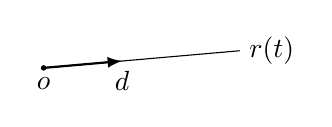
\begin{tikzpicture}[]
		\coordinate[label=below:$\vtr{o}$] (o) at (0,0);
		\coordinate[label=below:$\vtr{d}$] (d) at (5:1);
		\coordinate[label=right:$\vtr{r}(t)$] (rt) at (5:2.5);
		\fill[] (o) circle (1pt);
		\draw[] (o) -- (rt);
		\draw[-latex,thick] (o) -- (d);
	\end{tikzpicture}
\end{center}
\begin{compactdesc}
\item[\lp{Sphere}] Equation:
	\begin{gather*}
		\norm{\vtr{x}-\vtr{c}}^2-r^2=0,
	\end{gather*}
	with $\vtr{x}$ point of interest, $\vtr{c}$ center, $r^2$ radius. Insert ray equation \ref{eq:rayeq}. Solve for $t$
	\begin{gather*}
		\norm{\vtr{o}+t\vtr{d}-\vtr{c}}^2-r^2=0.
	\end{gather*}
	\item[\lp{Triangle}] Barycentric coordinates
		\begin{gather*}
			\vtr{x}=s_1\vtr{p}_1+s_2\vtr{p}_2+s_3\vtr{p}_3.
		\end{gather*}
		Intersect with triangle's plane
		\begin{gather*}
			(\vtr{o}+t\vtr{d}-\vtr{p}_1)\cdot \vtr{n}=0
		\end{gather*}
		\begin{align*}
			t&=-\frac{(\vtr{o}-\vtr{p}_1)\cdot \vtr{n}}{\vtr{d}\cdot \vtr{n}},\quad\text{where},\\
			n&=(\vtr{p}_2-\vtr{p}_1)\times (\vtr{p}_3-\vtr{p}_1).
		\end{align*}
		Compute $s_i$, test
		\begin{gather*}
			s_1+s_2+s_3=1,\quad 0\leq s_i\leq 1.
		\end{gather*}
		\section{Shading}
		Physically exact shading too costly. 
	\item[\lp{Simplifying assumptions}]\mbox\\
		\begin{enumerate*}[label=\protect\circled{\arabic*},itemjoin=]
			\item Surface reflectance: diffuse, specular, ambient, transparency terms\\
			\item Shadows: Shadow rays to determine if a hit point is in shadow or not.\\
		\end{enumerate*}
\section{Extensions}
	\item[\lp{Refraction}] \mbox\\
		\pgr{5-2_RayTracing}{26}{-1.7}{-1.35}{1.7}{0.57}
	\item[\lp{multiple lights}]
	\item[\lp{Area lights for soft shadows}] Multiple shadow rays to sample area light source.
	\item[\lp{Motion blur}] Sample objects and intersect in time.
		\begin{center}
			\begin{tikzpicture}[]
				\node[circle,fill=subsectionlinecolor,minimum size=1cm,label=below:${t=0}$] (c1) at (0,0) {};
				\node[circle,draw,dashed,minimum size=1cm,label=below left:${t=-1}$] (c2) at (-0.3,0) {};
				\node[circle,draw,dashed,minimum size=1cm,label=below right:${t=1}$] (c3) at (0.3,0) {};
			\end{tikzpicture}
		\end{center}
	\item[\lp{Depth of field}] Makes the final image look like a picture taken by a camera with a focus. Simulate a lens with a certain focal length.
\section{Acceleration}
\item[\lp{Cost}]
$\mathcal{O}(\#\text{rays}\times \#\text{objects})$. $50K$ trees each with $1M=50B$ $\to$ 594 years!
\item[\lp{Solution}] Uniform grids, space partitioning trees. $\to$ $\SI{10}{\minute}$ $\to$ $300000000\times$ speedup
\item[\lp{Uniform grids - preprocessing}]\mbox\\
		\pgr{5-2_RayTracing}{40}{1.2}{-1.2}{3.0}{0.47}
	\begin{enumerate*}[label=\protect\circled{\arabic*},itemjoin=]
		\item Compute bounding box\\
		\item set grid resolution\\
		\item rasterize objects\\
		\item store references to objects
	\end{enumerate*}
	\item[\lp{Uniform grids - advantages}] Fast to build, easy to code
	\item[\lp{Uniform grids - disadvantages}] Non-adaptive to scene geometry
	\item[\lp{Uniform grids - example: tea pot}] Brute force: 6321 intersections tests per ray. Uniform grid: 44.86 intersectio tests per ray.
	\item[\lp{Space partitioning trees}]\mbox\\
		\pgr{5-2_RayTracing}{43}{-2.7}{-1.35}{2.7}{0.57}
\end{compactdesc}
